%!TEX root = ../template.tex
%%%%%%%%%%%%%%%%%%%%%%%%%%%%%%%%%%%%%%%%%%%%%%%%%%%%%%%%%%%%%%%%%%%
%% chapter1.tex
%% NOVA thesis document file
%%
%% Chapter with introduction
%%%%%%%%%%%%%%%%%%%%%%%%%%%%%%%%%%%%%%%%%%%%%%%%%%%%%%%%%%%%%%%%%%%

\typeout{NT FILE chapter2.tex}%

\chapter{Background}

\section{Propositional Logic}
\label{chap:prop}
Logic in general is defined as the study of the principles of reasoning. \gls{PL} is a branch of logic that focuses on the study of propositions and their relationships. The goal of logic in computer science is to create languages that help us represent situations we deal with as computer scientists. These languages allow us to think about and analyze these situations in a structured way. By using logic, we can build clear and valid arguments about these situations, ensuring they make sense and can be tested, defended, or even carried out by a machine~\cite{huth_2004_logic}.

Propositions are the basic building blocks of \gls{PL}. A proposition is a declarative statement that has a truth value, which can be either true(denoted as T or 1) or false (denoted as F or 0), but not both.

\textbf{Examples of Propositions:}
\begin{itemize}
    \item "Today is friday."
    \item "It is raining."
    \item "If it is cold, then it is raining."
\end{itemize}

\subsection{Syntax}
\label{chap:prop-syntax}
To define a formal language, one must choose the alphabet of the language and establish the set of words that make up the language. These words are usually called formulas when the formal language is associated with a logic, as is the case here. The alphabet of the language is a set of symbols, and each formula is a finite sequence of symbols from the alphabet.

Symbols are used to represent propositions and the relationships between them. By convention, propositions are represented by lowercase letters (\(p\),\(q\),\(r\)) or by Greek letters (\(\phi\),\(\psi\),\(\gamma\)). The tables \ref{tab:logical_constants_and_prop_vars} and \ref{tab:logical_connectives} list all the logical constants, propositional variables, and logical connectives in \gls{PL}. 

\begin{table}[h!]
    \centering
    \resizebox{\textwidth}{!}{ 
    \begin{tabular}{|c|p{6cm}|p{8cm}|}
    \hline
    \textbf{Symbol} & \textbf{Name} & \textbf{Example} \\ \hline
    \(\top\) & Top  & \(\top\): "True" \\ \hline
    \(\bot\) & Bottom  & \(\bot\): "False" \\ \hline
    \(p\),\(q\),\(r\) & Propositions  & \(p\): "It is raining." \\ \hline
    \end{tabular}}
    \caption{Logical Constants and Propositional Variables}
    \label{tab:logical_constants_and_prop_vars}
\end{table}

\begin{table}[h!]
    \centering
    \resizebox{\textwidth}{!}{
    \begin{tabular}{|c|p{6cm}|c|p{8cm}|}
    \hline
    \textbf{Symbol} & \textbf{Name} & \textbf{Arity} & \textbf{Example} \\ \hline
    \(\neg\) & Not & 1 & \(\neg p\): "It is not raining." \\ \hline
    \(\land\) & And & 2 & \(p \land q\): "It is raining and it is cold." \\ \hline
    \(\lor\) & Or & 2 & \(p \lor q\): "It is raining or it is cold." \\ \hline
    \(\to\) & Implication & 2 & \(p \to q\): "If it is raining, then it is cold." \\ \hline
    \(\leftrightarrow\) & Equivalence & 2 & \(p \leftrightarrow q\): "It is raining if and only if it is cold." \\ \hline
    \end{tabular}}
    \caption{Logical Connectives}
    \label{tab:logical_connectives}
\end{table}

A well-formed formula (WFF) in \gls{PL} is defined recursively according to the following set of rules (\ref{tab:wff_rules}), which specify the conditions under which a formula is considered well-formed, and these rules build upon each other to allow for the construction of more complex logical expressions.

\begin{table}[h] 
\[
\left\{
\begin{array}{ll}
\alpha \text{ is WFF} & \text{,if } \alpha \text{ is a proposition,}\\
\neg \alpha \text{ is a WFF} & \text{,if } \alpha \text{ is a WFF,}\\
(\alpha \land \beta) \text{ is a WFF} & \text{,if } \alpha \text{ and } \beta \text{ are WFFs,}\\
(\alpha \lor \beta) \text{ is a WFF} & \text{,if } \alpha \text{ and } \beta \text{ are WFFs,} \\
(\alpha \rightarrow \beta) \text{ is a WFF} & \text{,if } \alpha \text{ and } \beta \text{ are WFFs,} \\
(\alpha \leftrightarrow \beta) \text{ is a WFF} & \text{,if } \alpha \text{ and } \beta \text{ are WFFs} \\
\end{array}
\right.
\]

\caption{Rules for Well-Formed Formulas in Propositional Logic}
\label{tab:wff_rules}
\end{table}

\textbf{Examples of WFF:}
\begin{itemize}
    \item \(\top\): "True".
    \item \((p \land q) \to r\): "If it is raining and it is cold, then it is snowing."
    \item \((p \to q) \land (q \to r)\): "If it is raining, then it is cold, and if it is cold, then it is snowing."
\end{itemize}

\subsection{Semantic}
To define a language, we also need to define its semantics. In \gls{PL}, this is not different, given a formula, we may want to determine its truth value. To do so, we must create an interpretation by assigning a truth value to each propositional symbol.
We say that a formula is satisfiable (SAT) over an interpretation if the interpretation satisfies the formula (it evaluates true in that interpretation). Otherwise, the formula is not satisfiable. Table \ref{tab:sat_rules} presents the inductive definition of SAT in \gls{PL}.


\begin{table}[h]
\[
\left\{
\begin{array}{ll}
    \alpha \text{ is SAT}  & \text{,if } \alpha \text{ is a proposition and its interpretation is true}, \\
    \neg \alpha \text{ is SAT} & \text{,if } \alpha \text{ is not SAT,} \\
    (\alpha \lor \beta) \text{ is SAT} & \text{,if either } \alpha \text{ or } \beta \text{ is SAT,} \\
    (\alpha \land \beta) \text{ is SAT} & \text{,if both } \alpha \text{ and } \beta \text{ are SAT,} \\
    (\alpha \rightarrow \beta) \text{ is SAT} & \text{,if whenever } \alpha \text{ is SAT, then } \beta \text{ is SAT,} \\
    (\alpha \leftrightarrow \beta) \text{ is SAT} & \text{,if both } \alpha \text{ and } \beta \text{ are either both SAT or both not SAT.}
\end{array}
\right.
\]

\caption{Inductive definition of SAT in \gls{PL}}
\label{tab:sat_rules}
\end{table}

A formula is said to be possible if there is an interpretation that satisfies it. A more specific type of a possible formula is the one that is valid, or tautological, which is satisfied by any interpretation.

\subsection{Equivalences}
\label{chap:prop-equivalences}
In \gls{PL}, we may want to determine if two formulas are logically equivalent (\(\equiv\)), which occurs when, for all possible interpretations, both formulas always have the same truth values. There are several methods to check whether two logical formulas are equivalent:

\begin{itemize}
    \item \textbf{Truth tables:} A truth table examines all possible interpretations for the propositions involved. To construct a truth table, we need to list all propositions, enumerate all possible truth value interpretations for those propositions, and evaluate the truth values of the formulas for each interpretations. If the results match in all rows, both formulas are equivalent. The number of interpretations can easily scale up depending on the number of propositions involved. For example, if we consider \( n \) propositions, the total number of rows will be \( 2^n \). This is not a feasible method for evaluating large expressions due to the exponential growth in the number of rows. However, for smaller expressions, truth tables are effective. The table \ref{tab:eq_truth_table} demonstrates \( p \to q \equiv \lnot p \lor q \).
   \begin{table}[h]
            \centering
            \[
            \begin{array}{|c|c|c|c|}
            \hline
            p & q & p \to q & \lnot p \lor q \\ 
            \hline
            T & T & T & T \\ 
            T & F & F & F \\ 
            F & T & T & T \\ 
            F & F & T & T \\ 
            \hline
            \end{array}
            \]
            \caption{Truth table showing the equivalence between \(p \to q\) and \(\lnot p \lor q\).}
            \label{tab:eq_truth_table}
            \end{table}     

    \item \textbf{Algebraic Manipulation:} This approach relies on a set of rules, known as logical equivalences, that can be used to manipulate expressions, similar to how it works in mathematics. By applying these equivalences, we can transform one logical expression into another that is logically equivalent, meaning both expressions have the same truth value in every scenario. Here is the list of some well-known logical equivalences: 
    
    \begin{itemize}
        \item \textbf{Identity Law:} \( p \land \top \equiv p \) and \( p \lor \bot \equiv p \)
        \item \textbf{Domination Law:} \( p \land \bot \equiv \bot \) and \( p \lor \top \equiv \top \) 
        %\item \textbf{Idempotent Law:} \( p \land p \equiv p \)
        %\item \textbf{Negation Law:} \( p \land \neg p \equiv \bot \)
        %\item \textbf{Double Negation Law:} \( \neg (\neg p) \equiv p \)
        \item \textbf{Commutative Law:} \( p \land q \equiv q \land p \)
        \item \textbf{Associative Law:} \( (p \land q) \land r \equiv p \land (q \land r) \)
       % \item \textbf{Distributive Law:} \( p \land (q \lor r) \equiv (p \land q) \lor (p \land r) \) and \( p \lor (q \land r) \equiv (p\lor q) \land (p \lor r) \)
        %\item \textbf{Absorption Law:} \( p \land (p \lor q) \equiv p \)
        %\item \textbf{Implication Law:} \( p \to q \equiv \neg p \lor q \)
        \item \textbf{DeMorgan’s Law:} \( \neg (p \land q) \equiv (\neg p) \lor (\neg q) \) and \( \neg (p \lor q) \equiv (\neg p) \land (\neg q) \)
    \end{itemize}
        
\end{itemize}

\section{First-Order Logic}
\label{chap:fol}
Another branch of logic is \gls{FOL}, also known as predicate logic. Unlike \gls{PL}, which focuses solely on simple declarative statements, first-order logic extends this by introducing quantifiers, predicates, variables, constants, and functions. These additional components allow us to express more complex declarative sentences, capturing relationships between objects and their properties in a specified context~\cite{huth_2004_logic, gouveia_lgica}.

\textbf{Examples of First-Order Sentences:}
\begin{itemize}  
    \item "There's a black cat that likes baths." 
    \item "John is a friend of Mary." 
    \item "If a variable is an integer and positive, then it is greater than zero." 
\end{itemize}  

\subsection{Syntax}
\label{chap:fol-syntax}
\gls{FOL} uses the same syntax as \gls{PL} but adds more features to make it more expressive. It introduces quantifiers that allow us to generalize or specify expressions, making it possible to express universal truths or existential statements. Quantifiers also enable the introduction of variables within a certain domain. Predicates that are used to express properties or relationships, allowing \gls{FOL} to capture facts about objects and their interactions. They are always denoted with a capital letter, return a truth value, and can have different arities. Similar to predicates, \gls{FOL} includes functions that represent mappings or computations. Functions are represented with lowercase letters, and their return value is a specific value in the domain.

\begin{table}[h!]
    \centering
    \resizebox{\textwidth}{!}{
    \begin{tabular}{|c|p{4cm}|p{10cm}|} 
    \hline
    \textbf{Symbol} & \textbf{Name} & \textbf{Example} \\ \hline
    \(x, y, z\) & Variables & \(x\): "An individual object" \\ \hline
    \(black\) & Constants & \(black\): "Value that is fixed" \\ \hline
    \(Cat(x)\) & Predicates & \(Cat(x)\): "True if \(x\) is a cat" \\ \hline
    \(color(x)\) & Functions & \(color(x) = \text{black}\): "The color of \(x\) is black" \\ \hline
    \end{tabular}}
    \caption{Examples of variables, constants, predicates, and functions in \gls{FOL}}
    \label{tab:pred_var_const_fun}
\end{table}

\begin{table}[h!]
    \centering
    \resizebox{\textwidth}{!}{
    \begin{tabular}{|c|p{4cm}|p{10cm}|}
    \hline
    \textbf{Symbol} & \textbf{Name} & \textbf{Example} \\ \hline
    \(\forall\) & Universal  & \(\forall x \, (Cat(x) \rightarrow Mammal(x))\): "All cats are mammals" \\ \hline
    \(\exists\) & Existential   & \(\exists x \, (Cat(x) \land color(x) = \text{black} \land LikesBaths(x))\): "There's a black cat that likes baths" \\ \hline
    \end{tabular}}
    \caption{Quantifiers in \gls{FOL}}
    \label{tab:quant}
\end{table}

We can extend the definition of a \gls{WFF} from \gls{PL} to represent a \gls{WFF} in \gls{FOL}. To accomplish this, we must first introduce a new concept known as a term. A term is an expression that represents a specific value in the domain. The tables \ref{tab:term_rules} and \ref{tab:fol_wff_rules} show a simplified version of defining a \gls{WFF} within \gls{FOL}.

\begin{table}[h]
    \centering
    \[
    \left\{
    \begin{array}{ll}
    c \text{ is a term} & \text{, if } c \text{ is a constant,} \\
    x \text{ is a term} & \text{, if } x \text{ is a variable,} \\
    %t_1 \mathbin{\{+, -, \times, /\}} t_2 \text{ is a term} & \text{, if } t_1 \text{ and } t_2 \text{ are terms,} \\
    f(t_1, t_2, \dots, t_n) \text{ is a term} & \text{, if } f \text{ is a function with arity } n \text{ and } t_1, t_2, \dots, t_n \text{ are terms.}
    \end{array}
    \right.
    \]
    \caption{Rules for Terms in \gls{FOL}}
    \label{tab:term_rules}
\end{table}

\begin{table}[h]
    \centering
    \[
    \left\{
    \begin{array}{ll}
    P(t_1, t_2, \dots, t_n) \text{ is a WFF} & \text{, if } P \text{ is a predicate with arity } n \text{ and } t_1, t_2, \dots, t_n \text{ are terms,} \\
    \neg \alpha \text{ is a WFF} & \text{, if } \alpha \text{ is a WFF,} \\
    \forall x \, \alpha \text{ is a WFF} & \text{, if } \alpha \text{ is a WFF and } x \text{ is a variable,} \\
    \exists x \, \alpha \text{ is a WFF} & \text{, if } \alpha \text{ is a WFF and } x \text{ is a variable,} \\
    %t_1 \mathbin{\{=, \neq, <, \leq, >, \geq\}} t_2 \text{ is a WFF} & \text{, if } t_1 \text{ and } t_2 \text{ are terms,} \\
    (\alpha \mathbin{\{\land, \lor, \rightarrow, \leftrightarrow\}} \beta) \text{ is a WFF} & \text{, if } \alpha \text{ and } \beta \text{ are WFFs.}
    \end{array}
    \right.
    \]
    \caption{Rules for Well-Formed Formulas in \gls{FOL}}
    \label{tab:fol_wff_rules}
\end{table}
    
\subsection{Semantic}
As in \gls{PL}, we must understand how semantics work in \gls{FOL}. Unlike \gls{PL}, in \gls{FOL}, an interpretation structure is a pair. The first element is the domain, and the second is a function, that assigns an application to functions and predicates. Additionally, an assignment of variables is a function that maps each variable to a specific element of the universe. Similarly to \gls{PL}, we say that a formula is SAT over an interpretation and an assignment, if the interpretation satisfies the formula (it evaluates true in that interpretation). Otherwise, the formula is not satisfiable. Table \ref{tab:sat_rules} presents the inductive definition of SAT in \gls{FOL}.

As in Propositional Logic \gls{PL}, the concepts of possibility, validity, and tautology are also applied in \gls{FOL}.

\begin{table}[h]
\[
    \left\{
    \begin{array}{ll}
        \alpha \text{ is SAT}  & \text{,if } \alpha \text{ is a predicate and its interpretation is true}, \\
        \neg \alpha \text{ is SAT} & \text{,if } \alpha \text{ is not SAT,} \\
        (\alpha \lor \beta) \text{ is SAT} & \text{,if either } \alpha \text{ or } \beta \text{ is SAT,} \\
        (\alpha \land \beta) \text{ is SAT} & \text{,if both } \alpha \text{ and } \beta \text{ are SAT,} \\
        (\alpha \rightarrow \beta) \text{ is SAT} & \text{,if whenever } \alpha \text{ is SAT, then } \beta \text{ is SAT,} \\
        (\alpha \leftrightarrow \beta) \text{ is SAT} & \text{,if both } \alpha \text{ and } \beta \text{ are either both SAT or both not SAT,} \\
        \forall x \, \alpha \text{ is SAT} & \text{,if for every element } u \in \text{ Universe, } \alpha \text{ is SAT when assigning } u \text{ to } x. \\
        \exists x \, \alpha \text{ is SAT} & \text{,if for some element } u \in \text{ Universe, } \alpha \text{ is SAT when assigning } u \text{ to } x. \\
    \end{array}
    \right.
\]


    \caption{Inductive definition of SAT in \gls{FOL}}
    \label{tab:sat_rules}
    \end{table}

\subsection{Equivalences}
Checking the equivalence of two expressions can be considerably more complicated in \gls{FOL} compared to \gls{PL}. \gls{FOL} is way more expressive and is not easy to guaratee that for all interpretations in both expressions the truth value is the same. In fact, there is no algorithm that can prove the equivalence of all expressions. This problem is considered undecidable and was proven by Alan Turing~\cite{turing_1936_on}. But there are some approaches that can be used to solve some kind of equivalences:

\begin{itemize}
    \item \textbf{Contradiction:} To demonstrate by contradiction, we assume the negative of the expression and try to derive a contradiction from that assumption. If the assumption results in an absurdity, the original assertion must be valid.
    \item \textbf{Algebraic Manipulation:} This approach works the same way as the one described in \gls{PL}. By applying these rules, we can transform one logical expression into another that is logically equivalent, meaning both expressions have the same truth value in every scenario. Here is the list of some well-known logical equivalences in \gls{FOL}:

    \begin{itemize}
        \item \textbf{Quantifier Negation:} \( \neg \forall x P(x) \equiv \exists x \neg P(x) \) and \( \neg \exists x P(x) \equiv \forall x \neg P(x) \)
        %\item \textbf{Universal Instantiation:} \( \forall x P(x) \equiv P(a) \) (for some constant \( a \))
        %\item \textbf{Existential Generalization:} \( P(a) \equiv \exists x P(x) \) (for some constant \( a \))
        %\item \textbf{Universal Generalization:} \( P(a) \equiv \forall x P(x) \) (if \( a \) is arbitrary)
        %\item \textbf{Existential Instantiation:} \( \exists x P(x) \equiv P(a) \) (for some constant \( a \), where \( a \) is a new constant)
        \item \textbf{Universal Distribution:} \( \forall x (P(x) \land Q(x)) \equiv \forall x P(x) \land \forall x Q(x) \)
        \item \textbf{Existential Disjunction:} \( \exists x (P(x) \lor Q(x)) \equiv \exists x P(x) \lor \exists x Q(x) \)

    \end{itemize}

\end{itemize}  

\section{Natural Deduction} 

\label{chap:prop-deduction}
A key task in Logic is to determine whether an expression \(\phi\) is a semantic consequence of a set of formulas \(\Gamma\), denoted by \(\Gamma \vdash \phi\). Given a set of premises and a conclusion, the conclusion is considered a semantic consequence of the premises if, for every interpretation of the propositions, whenever the interpretation satisfies all the premises, it must also satisfy the conclusion. In other words, if the set of premises is true, then the conclusion must also be true. 

To determine if an expression is a semantic consequence of a set of formulas, one can use a deduction system. There are two ways to approach a deduction system: the semantic approach looks at what the formulas mean in different ways, and the syntactic approach looks at how to use symbols in a deductive system~\cite{gouveia_lgica}. There are numerous deductive systems in logic, some of the most well-known being  resolution, tableau and natural deduction, but in this thesis we will concentrate on the natural deduction system.

Natural deduction is a type of syntactic deduction system that uses a pre-defined set of rules, called inference rules. By applying inference rules to the premises, we hope to get some more formulas, and by applying more inference rules to those, to eventually reach the conclusion~\cite{huth_2004_logic}.

There are many styles to represent these proofs. For example, the Fitch style uses a linear structure, with deeper indentation levels to represent assumptions or intermediate steps in the proof, while the tree style organizes the proof in a tree-shaped structure. In this thesis, we will focus on the tree-style representation. 

These tree-shaped structures, also known as deduction trees, represent proofs and are built starting from individual trees and successively applying rules of inference. The rules are identified on the right-hand side of the fractions. There are 3 different types of rules: introduction (\(I\)), which creates more complex formulas from simpler ones; elimination (\(E\)), which does the opposite; and absurdity (\(\bot\)), which derives any conclusion from a contradiction. Table \ref{tab:inf_rules} presents some examples of inference rules.

\begin{table}[h]
\[
\begin{array}{c c c}
\frac{\overset{\displaystyle \mathcal{D}_1\strut}{\displaystyle \varphi\strut} \quad \overset{\displaystyle \mathcal{D}_2\strut}{\displaystyle \psi\strut}}{\displaystyle \varphi \land \psi\strut} \quad (\land I) & 
\frac{\displaystyle \overset{\displaystyle \mathcal{D}\strut}{\varphi \land \psi\strut}\strut}{\displaystyle \varphi\strut} \quad (\land E_r) & 
\frac{\overset{\displaystyle[\neg\varphi]^m\strut}{\overset{\displaystyle\mathcal{D} \strut} {\displaystyle\bot 
\strut}}}{\displaystyle \varphi\strut} \quad (\bot, m) \\[10pt]
\textbf{Conjunction Introduction} & \textbf{Conjunction Elimination, right} & \textbf{Absurdity} \\[10pt]

\frac{\overset{\displaystyle [\varphi]^m\strut}{\overset{\displaystyle \mathcal{D}\strut}{\displaystyle\varphi\strut}\strut}\strut}{\displaystyle \varphi \to \psi\strut} \quad (\to I, m) & 
\frac{\overset{\displaystyle \mathcal{D}_1\strut}{\displaystyle \varphi\strut} \quad \overset{\displaystyle \mathcal{D}_2\strut}{\displaystyle \neg \varphi\strut}}{\displaystyle \bot\strut} \quad (\neg E) & 
\frac{\overset{\displaystyle [\varphi]^m\strut}{\overset{\displaystyle \mathcal{D}\strut}{\displaystyle\bot \strut}\strut}\strut}{\displaystyle \neg \varphi\strut} \quad (\neg I, m) \\[10pt]
\textbf{Implication Introduction} & \textbf{Negation Elimination} & \textbf{Negation Introduction} \\[10pt]
\end{array}
\]

\caption{Example of inference rules in Natural Deduction}
\label{tab:inf_rules}
\end{table}
Each rule has its own characteristic and can only be applied under certain circumstances. Some add new hypotheses that must be closed and others not. For instance, the Implication Introduction rule introduces a new hypothesis containing the antecedent of the implication, which can then be used to close the proof. Another example is the Conjunction Introduction rule that requires proving the left and right sides of the conjunction.

Individual trees are constructed from nodes, which are formulas. The formulas at the leaves are called hypotheses and are associated with marks (numbers). The formula at the root is the conclusion of the proof. Marks are used to identify the hypotheses that are given or derived from the rules. We call a closed hypothesis if its mark is used in a rule of the tree otherwise, it is said to be open. The table below illustrates the procedure of a basic proof where we aim to prove: \{\(\psi\)\} \( \vdash \varphi \to (\psi \land \varphi) \).

\begin{table}[h!]
    \[
    \begin{array}{c@{\hspace{1cm}}c}
            \frac{\displaystyle \psi \land \varphi\strut}{\displaystyle \varphi \to (\psi \land \varphi)\strut} \quad (\to I, 2) &
            \frac{\displaystyle\frac{\displaystyle \psi^1 \quad \varphi^2\strut}{\displaystyle \psi \land \varphi\strut}\quad (\land I)\strut}{\displaystyle \varphi \to (\psi \land \varphi)\strut} \quad (\to I, 2)\\[10pt]
            \textbf{First step} & \textbf{Second step} \\
    \end{array}
      \]
    \caption{Example of a deduction tree proving \{\(\psi\)\} \( \vdash \varphi \to (\psi \land \varphi) \).}
    \label{tab:proof-tree-part2}
\end{table}

Building these proofs can be done in a variety of ways: bottom-up by starting from the conclusion and top-down by starting from the premises or open clauses. If we consider a bottom-up solution, the first step is to apply the Implication Introduction rule. From this rule, we derive a new hypothesis (\(\varphi\)), which we will mark with the number two, since we already have a premise marked with the number one. At this point in the proof, we have \(\displaystyle \psi \land \varphi\) open. The second step is to apply the Conjunction Introduction rule, subsequently, both expressions in the leaves can now be closed with marks one and two, respectively. With no leaves left containing open hypotheses, the proof is declared complete when all necessary hypotheses have been closed and the desired conclusion is present at the root of the tree. So we proved \{\(\psi\)\} \( \vdash \varphi \to (\psi \land \varphi) \).

In logic courses, students often struggle the most with these types of exercises. Some steps in the proofs are not immediately obvious, and trees can become quite large with many branches. Becoming proficient requires significant exposure and practice. The following schema illustrates a more complex example of a proof.
\begin{table}[h!]
    \centering
    \[
    \frac{\displaystyle \frac{\displaystyle \frac{
    \displaystyle \neg (\varphi \lor \psi)^1 \quad \displaystyle \frac{\psi^2}{(\varphi \lor \psi) \strut} \quad (\lor I_l) \strut}
    {\displaystyle \bot \strut} \quad (\displaystyle \neg E)\strut} {\displaystyle \neg \psi \strut} \quad (\neg I, 2) \strut}
    {\neg (\varphi \lor \psi) \to \neg \varphi \strut} \quad (\to I, 1)
    \]
    \caption{Example of a more complex deduction tree proving \( \vdash \neg (\varphi \lor \psi) \to \neg \varphi \).}
    \label{tab:proof-tree1}
\end{table}
    

%Looking at the example in \ref{tab:proof-tree}, if we consider a bottom-up solution, the first step is to apply the Implication Introduction rule to the conclusion. By doing so, we add the left part of the implication as a hypothesis and assign it a mark, numbered 1. Next, the Negation Introduction rule (\(\neg I\)) is applied. From this rule, \(\psi\) is obtained and added to our list of hypotheses, with a fresh mark assigned, numbered 2. Negation Elimination rule (\(\neg E\)) then is followed. This rule requires an expression and its negation to be applied. The hypothesis introduced in the first rule serves this purpose. The left side of the rule is closed. To complete the proof, the right side must also be closed. As a final step, the Disjunction Introduction rule on the left (\(\lor I_l\)) is applied, and the proof is closed using hypothesis 2.

\section{Proof Assistants}
Proof assistants are software tools designed to help their users formalize programs or mathematical concepts and prove theorems about them~\cite{andersschlichtkrull_2015_formalization}. Besides that, they can check step-by-step that the proof is correct according to a set of axioms and rules ensuring its correctness. Several proof assistants can also automate some steps, or even the full proof. Libraries that provide reusable theorems, definitions, and strategies can extend them, enhancing efficiency and simplifying complex proofs.

Proof assistants can have a big impact in education, particularly for teaching mathematical reasoning and formal semantics. This type of tool can be used in Logic, for example, to help in constructing proofs in deduction systems. Some tools have a user-friendly interface, so the user can navigate through the steps of the proof to see the state on the step, can display information about the current goals, and provide little hints/suggestions about the steps to follow.

In the following sections, we present two examples of proof assistants that can be used in natural deduction.

\subsection{Isabelle/HOL}
Isabelle is a generic framework for interactive theorem proving. Isabelle/HOL is a large application within the generic framework that focuses on higher order logic (HOL). It includes a wide range of tools for logic-specific tasks and a large theory library~\cite{wenzel_the,blanchette_automatic}. Isabelle/HOL is based on tactic functions that manipulate the proof state. These tactics can either solve a proof goal directly or break it into smaller subgoals. For instance, Blast is a first-order tableau prover, and Metis is a resolution prover.

Sledgehammer is an extremely powerful tool in Isabelle/HOL, which connects it with external provers by sending its problems to remote servers, increasing the efficiency of the prover. Additionally, it can automate proofs by utilizing various tactics that external provers have discovered. This automatization can be useful when combined with large proofs, as it can omit certain steps by using tactics. However, it may also hide some of the underlying reasoning behind the proof, making it harder for users to understand the intermediate steps. Since this tool cannot provide a full proof or a step-by-step resolution, it may not be suitable for developing our feedback system for natural deduction exercises.

However, Isabelle/HOL has tools for making counterexamples. For example, Nitpick uses a solver to systematically look for edge cases, and QuickCheck creates tests at random to test the properties of the expressions. These tools can be used in our feedback system to provide counterexamples to students, assisting them in identifying errors in their reasoning and improving their comprehension of the exercises. Figure \ref{img:isabelle-counter} shows an example of how these tools are used and the corresponding counterexample found.
\begin{figure}[htbp]
    \centering
    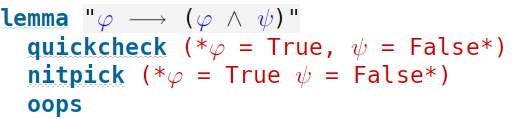
\includegraphics[width=0.5\linewidth]{Isabelle-counter}
    \caption{Example of code in Isabelle testing Nitpick and Quickcheck.}
    \label{img:isabelle-counter}
\end{figure}


    
\subsection{Lean}
Lean is a functional programming language that can be used as an interactive theorem prover~\cite{programming}. The structure of the proofs is very similar to the one presented in~\ref{chap:prop-deduction}, where it is possible to use rules defined in natural deduction, in contrast to Isabelle/HOL. Figure \ref{img:lean_example} shows an example of a natural deduction proof in Lean style, and \ref{tab:lean_example} demonstrates its representation in a tree style.

\begin{figure}[htbp]
    \centering
    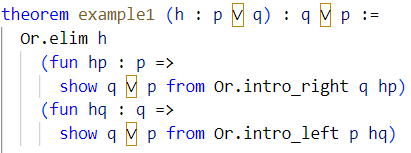
\includegraphics[width=0.5\linewidth]{Lean_example}
    \caption{Example of code in Lean proving \(\{p \lor q\} \models q \lor p \).}
    \label{img:lean_example}
\end{figure}
\begin{table}[h!]
    \centering
        \[
            \frac{ {\displaystyle {p \lor q}^1 
            \quad \quad \displaystyle \frac{\displaystyle p^2}{q \lor p \strut} (\lor I_l) \strut}
            \quad \quad \displaystyle \frac{\displaystyle q^3}{q \lor p \strut} (\lor I_r) \strut}
            {\displaystyle q \lor p \strut} \quad (\vee E, 2, 3)
          \]
          \caption{Example of a deduction tree proving \(\{p \lor q\} \models q \lor p \).}
          \label{tab:lean_example}
      \end{table}

Lean also has a tool to automate proofs called Aesop~\cite{leanprovercommunity_2021_github}. Unlike Isabelle/HOL, Aesop can provide a step-by-step proof, but not in the format presented above. The generated proof uses different tactics that are genereraly not easy to directly map to natural deduction rules. However, Aesop alows users to define their own rules/tactics to help with automation. It is possible to restrict the domain of the rules used in the automation process. Perhaps by defining the set of all natural deduction rules, we could achieve the desired output, enabling the generation of proofs using only valid rules. If we successfully accomplish this, we will have a reliable method for implementing our feedback.

Another interesting feature of Aesop is that it allows the user to use part of their proof to generate the rest of it when possible.




